\documentclass{article}
\usepackage{float}
\usepackage{amsmath}
\usepackage{amssymb}
\usepackage{graphicx}

\usepackage[top=1in, bottom=1.25in, left=1.25in, right=1.25in]{geometry}

\newcommand{\bs}[1]{\boldsymbol{#1}}
\newcommand{\ul}[1]{\underline{#1}}
\newcommand{\ulbs}[1]{\underline{\boldsymbol{#1}}}
\newcommand{\bsbar}[1]{\boldsymbol{\bar{#1}}}
\newcommand{\ulbsbar}[1]{\underline{\boldsymbol{\bar{#1}}}}
\newcommand{\vbs}[0]{\boldsymbol{v}}

\begin{document}

\section{Perfectly inelastic collision}
Two bodies A and B, with known masses and velocities collide and merge with each other, resulting in the body C. The problem is to find the velocity of the body C.

\begin{figure}[h]
	\centering
	{\includegraphics{figures/perfectly_inelastic_collision.pdf}}
	\caption{Perfectly inelastic collision.}\label{fig:perfectly_inelastic_collision}
\end{figure}

Conservation of linear momentum:
\begin{equation*}
m_A\vbs_A + m_B\vbs_B = m_C\vbs_C
\end{equation*}
It is assumed that all bodies have the same density $\rho$ and thickness $t$, i.e. $m = \rho t A$, where $A$ is the area. Hence, we have
\begin{equation*}
A_A\vbs_A + A_B\vbs_B = A_C\vbs_C
\end{equation*}
Since the bodies merge with each other, $A_C = A_A + A_B$, thus
\begin{equation*}
A_A\vbs_A + A_B\vbs_B = (A_A + A_B)\vbs_C
\end{equation*}
Solving for $\vbs_C$, we obtain
\begin{equation}
\label{eq:perfectly_inelastic_collision}
\vbs_C = \frac{A_A}{A_A + A_B}\vbs_A + \frac{A_B}{A_A + A_B}\vbs_B
\end{equation}

\section{Ejection}
A body A with known velocity ejects a body B at a known velocity. We refer to the resulting form of body A (now with diminished mass), as A'. The problem is to find the velocity of the body A'.

\begin{figure}[h]
	\centering
	{\includegraphics{figures/ejection.pdf}}
	\caption{Ejection of mass.}\label{fig:ejection}
\end{figure}

Conservation of linear momentum:
\begin{equation*}
\begin{split}
m_A\vbs_A &= m_B\vbs_B + m_{A'}\vbs_{A'}
\Rightarrow
\\A_A\vbs_A &= A_B\vbs_B + A_{A'}\vbs_{A'}
\end{split}
\end{equation*}
Since $A_A = A_{A'} + A_B$, we get
\begin{equation*}
A_A\vbs_A = A_B\vbs_B + (A_A - A_B)\vbs_{A'}
\end{equation*}
Solving for $\vbs_{A'}$, we obtain
\begin{equation}
\vbs_{A'} = \frac{A_A}{(A_A - A_B)}\vbs_A - \frac{A_B}{(A_A - A_B)}\vbs_B
\end{equation}

\section{Partial merge}
Two bodies A and B, with known masses and velocities, A being the largest, collide and partially merge with each other such that the larger body A absorbs part of the smaller body B. The part of B that is absorbed by A is denoted as C. The result is an enlarged form of body A: A', and a diminished form of body B: B'. The problem is to find the velocities of the bodies A' and B'.

\begin{figure}[h]
	\centering
	{\includegraphics{figures/partial_merge.pdf}}
	\caption{Partial merge of two bodies.}\label{fig:partial_merge}
\end{figure}

We assume that C is released from body B without any impulse or energy transfer between B and C. Thus, the velocity of B is completely unaffected during the collision:
\begin{equation}
\vbs_{B'} = \vbs_B
\end{equation}
Furthermore, the body C will travel with the velocity $\vbs_B$ and be absorbed by A in a perfectly inelastic collision. Thus, from Equation \ref{eq:perfectly_inelastic_collision} we obtain
\begin{equation}
\vbs_{A'} = \frac{A_A}{A_A + A_C}\vbs_A + \frac{A_C}{A_A + A_C}\vbs_B
\end{equation}


\end{document}
